\def\uds#1{#1}

\section{Optimization}
\label{sec:optimization}

We now describe in detail the optimization algorithm for the additive
convex regression stage.  The second decoupled concave regression stage
follows a very similar procedure.

Let $\bds{x}_{i}\in\mathbb{R}^{p}$ be the covariate, let $y_{i}$ be
the response and let $\epsilon_{i}$ be the mean zero noise. The
regression function $f(\cdot)$ we estimate is the sum of
univariate functions $f_{k}(\cdot)$ in each variable dimension and a scalar
offset $\mu$.  We impose additional constraints that each
function $f_{k}(\cdot)$ is convex function, which can be
represented by its supporting hyperplanes, i.e.,
\begin{equation}\label{hyper}
      f_{i'k} \geq f_{ik} + \beta_{ik}(x_{i'k}-x_{ik}) \quad
      \textrm{for all $i,i' = 1,\ldots, n$,}
\end{equation}
where $f_{ik}\coloneqq f_{k}(x_{ik})$ and $\beta_{ik}$ is the
subgradient at point $x_{ik}$. This apparently requires $O(n^2 p)$ constraints to
impose the supporting hyperplane constraints.
In fact, only $O(np)$
constraints suffice, since univariate convex functions are
characterized by the condition that the subgradient, which is a scalar, must
increase monotonically. This observation leads to the  optimization
\begin{equation}
\begin{split}
       \min_{f,\beta,\mu} & \;\; \frac{1}{2n}\sum_{i=1}^{n}
                     \Bigl( y_{i}-\mu - \sum_{k=1}^{p}f_{ik}\Bigr)^{2} 
                         + \lambda\sum_{k=1}^{p}\|f_k\|_{\infty} \\
       \textrm{subject to} &\;\; \textrm{for all $k=1,\ldots, p$:}\\
       & \;\; f_{(i+1)_k k} = f_{(i)_k k} +
       \beta_{(i)_k k}(x_{(i+1)_k k}-x_{(i)_k k}),\;\textrm{for $i=1,\ldots, n-1$}\\
       & \;\; \sum_{i=1}^{n}f_{ik}=0,\\
       & \;\; \beta_{(i+1)_k k} \geq \beta_{(i)_k k}\;\textrm{for $i=1,\ldots, n-1$}.
\end{split}
\label{np}
\end{equation}
Here $f_k$ denotes the vector $f_k = (f_{1k}, f_{2_k}\ldots, f_{nk})^T\in\reals^n$
and $\{(1)_k,(2)_k,\ldots,(n)_k\}$ are the indices in the sorted ordering
of the values of coordinate $k$:
\begin{equation}
x_{(1)_k k} \leq{} x_{(2)_k k} \leq \cdots \leq{} x_{(n)_k k}.
\end{equation}


We can solve for $\mu$ explicitly as  
$\mu = \frac{1}{n} \sum_{i=1}^n y_i = \bar{y}$.  This follows from the
KKT conditions
and the constraints $\sum_i f_{ki} = 0$.
It is easy to verify that the constraints in (\ref{np}) satisfy the
supporting hyperplane constraints, since
for all $j > i$
\begin{align*}
  f_{(j)_kk}-f_{(i)_kk}  & = \sum\limits_{t=i}^{j-1}(f_{(t+1)_kk}-f_{(t)_kk}) \\
   &= \sum\limits_{t=i}^{j-1}\beta_{(t)_kk}(x_{(t+1)_kk}-x_{(t)_kk}) \\
   &\geq \beta_{(i)_kk}\sum\limits_{t=i}^{j-1}(x_{(t+1)_kk}-x_{(t)_kk}) \\
  & = \beta_{(i)_kk}(x_{(j)_kk}-x_{(i)_kk}) 
\end{align*}
and for all $j < i$
\begin{align*}
f_{k(j)}-f_{k(i)} & =
    \sum\limits_{t=j}^{i-1}(f_{k(t)}-f_{k(t+1)}) \\
     & = \sum\limits_{t=j}^{i-1}\beta_{k(t)}(x_{k(t)}-x_{k(t+1)}) \\
     &\geq \beta_{k(i)}\sum\limits_{t=j}^{i-1}(x_{k(t)}-x_{k(t+1)}) \\
     & = \beta_{k(i)}(x_{k(j)}-x_{k(i)}).
\end{align*}


%\begin{SCfigure}
%\label{fig:outer_approximation}
%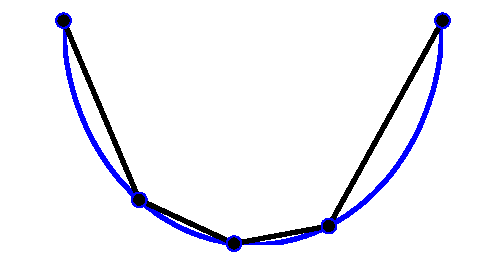
\includegraphics[width=0.3\textwidth]{figs/outer_approximation.pdf}
%\caption{With the 5 sample points $(X_i, h(X_i))$, the
%  black and the blue convex function represent equivalent fits. SCAM
%  chooses the inner piece-wise linear convex functions.}
%\end{SCfigure}

The sparse convex additive model optimization in (\ref{np}) is a quadratic program with
$O(np)$ variables and $O(np)$ constraints. 
Directly applying a QP solver for $f$ and $\beta$
is computationally expensive for relatively large
$n$ and $p$. However, notice that variables in different feature
dimensions are only coupled in the squared error term
$(y_{i}-\mu - \sum_{k=1}^{p}f_{ik})^{2}$. Hence, we can apply the block
coordinate descent method, where in each step we solve the following
QP subproblem for $\{f_k, \beta_k\}$ with the
other variables fixed. In matrix notation, the optimization is
\begin{align}
\begin{split}
\min_{ f_k, \beta_k, \gamma_k} \;\;& \frac{1}{2n} \| \uds{r}_k - \uds{f}_k \|_2^2 
     + \lambda \gamma_k \label{opt:1d_compact} \\
 \textrm{such that } & P \uds{f}_k = \diag(P \bds{x}_k)  \uds{\beta}_k \\
   & D \uds{\beta}_k \leq 0 \\
   & -\gamma_k \mathbf{1}_n \leq \uds{f}_k \leq \gamma_k \mathbf{1}_n   \\
   & \mathbf{1}_n^\tran \uds{f}_k = 0 
\end{split}
\end{align}
where $\uds{\beta}_k \in \R^{n-1}$ is the vector $\uds{\beta}_k =
(\beta_{1k}, \ldots, \beta_{(n-1)k})^T$, and
$\uds{r}_{k} \in \R^n$ is the residual vector $\uds{r}_{k} = (y_i -
\hat\mu - \sum_{k' \neq k} f_{ik'})^T$.
In addition, 
$P \in \R^{(n-1) \times n}$ is a permutation matrix where the $i$-th
row  is all zeros except for a $-1$ in position $(i)_k$ and a $1$ in
position $(i+1)_k$, and $D \in \R^{(n-2) \times (n-1)}$ is another
permutation matrix  where the $i$-th row is all zeros except for a $1$ 
in position $i$ and a $-1$ in position $i+1$.  We denote by
$\diag( v )$ the diagonal matrix with diagonal entries $v$.
The extra variable $\gamma_{k}$ is introduced to impose the
regularization penalty involving the $\ell_{\infty}$ norm.  

% \begin{equation}
% \label{eqn:opt_1d}
% \begin{split}
%        \min_{\bds{h}_{k\cdot},\bds{\beta}_{k\cdot},\gamma_{k}} &
%              \ \frac{1}{2n}\sum_{i=1}^{n}\Bigl((Y_{i}-\bar{Y}
%                 -\sum_{r\neq{k}}f_{ri})-f_{ki}\Bigr)^{2} 
%                       + \lambda\gamma_{k} \\
%         \textrm{such that} & \ f_{k(i+1)} = f_{k(i)} + \beta_{k(i)}(x_{k(i+1)}-x_{k(i)}),\\
%         &\ \beta_{k(i+1)} \geq \beta_{k(i)}, \ -\gamma_{k}\leq f_{ki}\leq\gamma_{k}\\
%         &\  \sum_{i=1}^{n}f_{ki}=0, \ (\forall i).
% \end{split}
% \end{equation}

This QP
subproblem involves $O(n)$ variables, $O(n)$ constraints and a sparse
structure, which can be solved efficiently using optimization
packages. In our experiments we use {\sc mosek} (\href{http://www.mosek.com/}{www.mosek.com}).  We cycle through
all covariates $k$ from $1$ to $p$ multiple times until convergence.
Empirically, we observe that the algorithm converges in only a few
cycles. We also implemented an ADMM solver for (\ref{np})
\citep{Boyd:admm}, but found
that it is not as efficient as this QP solver.

After optimization, the function estimates for an input vector $\bds{x}$ is, according to (\ref{hyper}),
\begin{equation}
\begin{split}
      \hat f(\bds{x}) & = \sum_{k=1}^{p} \hat f_k(x_{j})+ \hat \mu 
= \sum_{k=1}^{p}\max_{i} \bigl\{\hat f_{ik}+ \hat \beta_{ik}(x_{k}-x_{ik})\bigr\} +
      \hat \mu.
\end{split}
\end{equation} 

The univariate concave function estimation is a straightforward
modification of optimization~\ref{opt:1d_compact}. It is only
necessary to modify the linear inequality constraints so that the subgradients are
non-increasing: $\beta_{(i+1)_kk} \leq \beta_{(i)_kk}$.


\subsection{Alternative Formulation}
Optimization (\ref{np}) can be reformulated in terms of the 2nd derivatives, a form which we analyze in our theoretical analysis. The alternative formulation replaces the ordering
constraints $\beta_{k(i+1)} \geq \beta_{k(i)}$ with positivity
constraints, which simplifies theoretical analysis.
Define $d_{k(i)}$ as the second derivative:
$d_{k(1)} = \beta_{k(1)}$, and $d_{k(2)} =
\beta_{k(2)} - \beta_{k(1)}$. The convexity constraint is
equivalent to the constraint that $d_{k(i)} \geq 0$ for all $i >
1$.

It is easy to verify that $\beta_{k(i)} = \sum_{j \leq i} d_{k(j)}$ and 
\begin{align*}
f_k(x_{k(i)}) = & f_k(x_{k(i-1)}) + \beta_{k(i-1)}(x_{k(i)} - x_{k(i-1)}) \\
 =& f_k(x_{k1}) + \sum_{j < i} \beta_{k(j)} (x_{k(j)} - x_{k(j-1)}) \\
 =& f_k(x_{k1}) + \sum_{j < i} \sum_{j' \leq j} d_{k(j')} (x_{k(j)} - x_{k(j-1)})\\
 =& f_k(x_{k1}) + \sum_{j' < i} d_{k(j')} \sum_{i > j \geq j'} (x_{k(j)} - x_{k(j-1)}) \\
 =& f_k(x_{k1}) + \sum_{j' < i} d_{k(j')} (x_{k(i)} - x_{k(j')})
\end{align*}
We can write this more compactly in matrix notations.
\begin{equation*}
\begin{split}
\left[ \begin{array}{c}
f_k(x_{k1}) \\
... \\
f_k(x_{kn}) 
\end{array} \right] =
\left[ \begin{array}{ccc}
    |x_{k1} - x_{k(1)}|_+ & ... & |x_{k1} - x_{k(n-1)}|_+ \\
    ... & & \\
    |x_{kn} - x_{k(1)}|_+ & ... & |x_{kn} - x_{k(n-1)}|_+ 
\end{array} \right]
\left[ \begin{array}{c}
    d_{k(1)} \\
    ... \\
    d_{k(n-1)}
\end{array} \right] 
+ \mu_k \equiv \Delta_k d_k + \mu_k
\end{split}
\end{equation*}


Where $\Delta_k$ is a $n\times n-1$ matrix such that $\Delta_k(i,j) = |x_{ki} - x_{k(j)}|_+$, $d_k = (d_{k(1)} ,..., d_{k(n-1)})$, and $\mu_k = f_k(x_{k1})$. 

Because $f_k$ has to be centered, $\mu_k = - \frac{1}{n} \mathbf{1}_n^\tran \Delta_k d_k$, therefore:
\[
\Delta_k d_k + \mu_k \mathbf{1}_n = 
   \Delta_k d_k - \frac{1}{n} \mathbf{1}_n \mathbf{1}_n^\tran \Delta_k d_k = 
   \bar{\Delta}_k d_k 
\]
where $\bar{\Delta}_k \equiv \Delta_k - \frac{1}{n} \mathbf{1}_n \mathbf{1}_n^\tran \Delta_k$ is $\Delta_k$ with the mean of each column subtracted.

We can now reformulate (\ref{np}) as an equivalent optimization program with only centering and positivity constraints:
\begin{align}
\min_{d_k}& \frac{1}{2n} 
       \Bigl\| Y - \sum_{k=1}^p 
              \bar{\Delta}_k d_k \Bigr\|_2^2 
               + \lambda_n \sum_{k=1}^p \|\bar{\Delta}_k d_k \|_\infty   
     \label{opt:alternate_opt} \\
\trm{s.t. }  & d_{k(2)}, \ldots , d_{k(n-1)} \geq 0  	
               \qquad \trm{(convexity)} \nonumber 
\end{align}

The decoupled concave postprocessing stage optimization is again similar. Suppose $\hat{d}_k$'s are the output of optimization~\ref{opt:alternate_opt}, define $\hat{r} = Y - \sum_{k=1}^p \bar{\Delta}_k \hat{d}_k$. 
\begin{align}
\textrm{for all}&\textrm{ $k$ such that $\hat{d}_k = 0$: }  \nonumber \\
  \min_{c_k} & 
      \frac{1}{2n} \Bigl \| \hat{r} - \Delta_k c_k \Bigr \|_2^2
      + \lambda_n \| \Delta_k c_k \|_\infty 
      \label{opt:alternate_opt_concave}\\
 \trm{s.t.} & c_{k(2)}, \ldots, c_{k(n-1)} \leq 0 \qquad \trm{(concavity)} \nonumber
\end{align}

We can use either the off-centered $\Delta_k$ matrix or the centered $\bar{\Delta}_k$ matrix because the concave estimations are decoupled and hence suffer no identifiability problems.\\

\begin{remark}
in sparsistency analysis, we assume that $B$, an upper bound to $\| f^*_k \|_\infty$, is known and that we constrain our estimate $\hat{f}$ to obey the same boundedness condition, that is, for each $k$, we require that $\|\hat{f}_k\|_\infty \leq B$. This boundedness constraint can be easily added to our optimization program. In optimization~\ref{opt:alternate_opt}, we can enforce the boundedness condition by adding $p$ constraints: $\| \bar{\Delta}_k d_k \|_\infty \leq B$ for $k=1,...,p$. (similarly for optimization~\ref{opt:alternate_opt_concave}). We emphasize that we use the boundedness constraint only in our theoretical analysis; all of our experiments do not impose any boundedness condition.
\end{remark}


% DO NOT CHANGE; RefTex variables -minx

%%% Local Variables: ***
%%% mode:latex ***
%%% TeX-master: "paper.tex" ***
%%% End: ***